\section*{Test problems --- true functions and noise}

\begin{figure}[htbp]
\centering
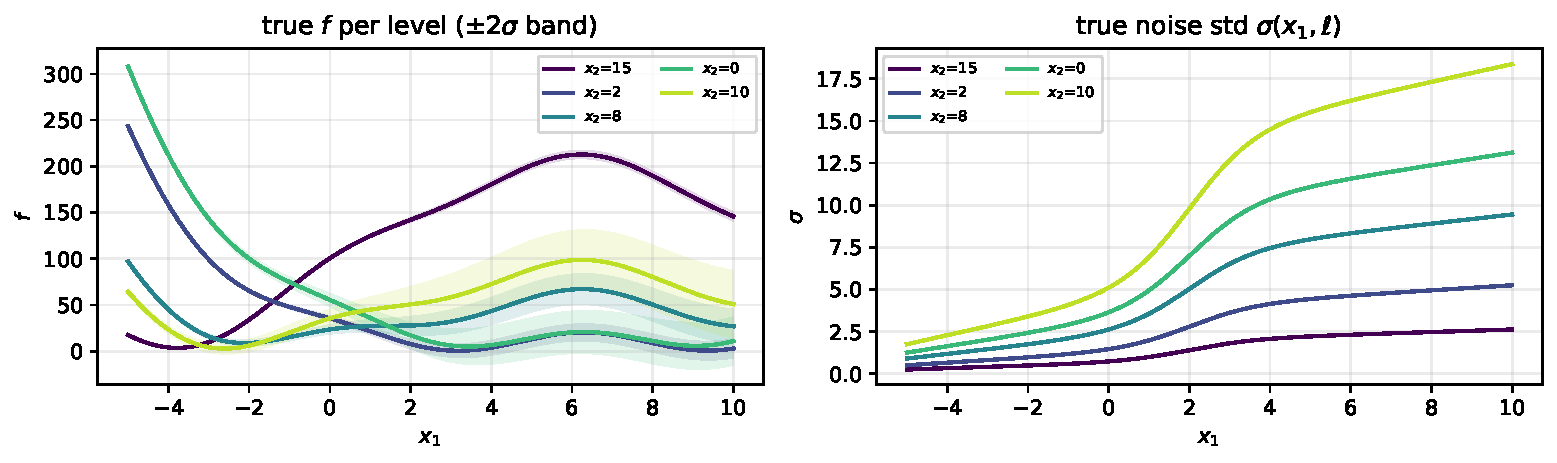
\includegraphics[width=0.9\linewidth]{figs/branin_truth.pdf}
\caption{Branin (v2 noise): true response per level with $\pm2\sigma$ noise band (left) and the
region-contrast noise std --- low-noise region, sigmoid step at $x_1\approx2$, high-noise
region --- with level multipliers $\{0.5,1.0,1.8,2.5,3.5\}$ (right).}
\end{figure}

\begin{figure}[htbp]
\centering
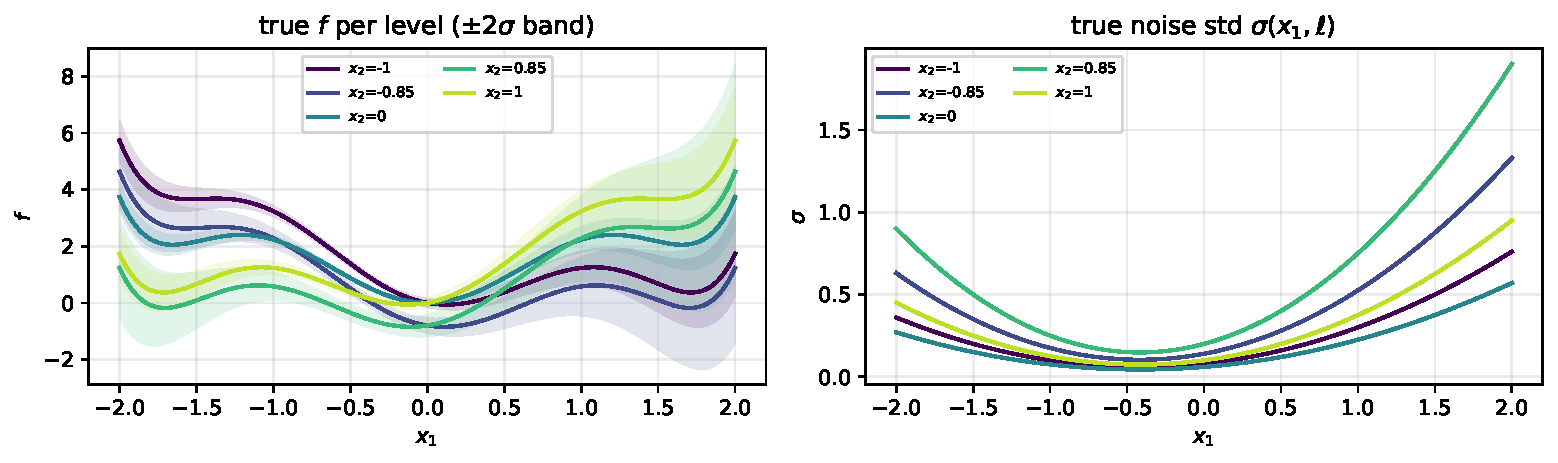
\includegraphics[width=0.9\linewidth]{figs/camel_truth.pdf}
\caption{Six-hump camel (v4 levels $\{-1.0,-0.85,0.0,0.85,1.0\}$, v4.3 polynomial noise
$(0.04+0.05x_1+0.06x_1^2)m(\ell)$): two pairs $\{1,2\}$ and $\{4,5\}$ (within-pair curve RMS
0.82) plus a middle bridge level 3 (1.16--1.27 from everything; cross-pair 1.97--2.32). The
30-seed camel tables were run under the earlier v4.0 noise $0.05e^{(0.4x_1)^2}m(\ell)$.}
\end{figure}

\begin{figure}[htbp]
\centering
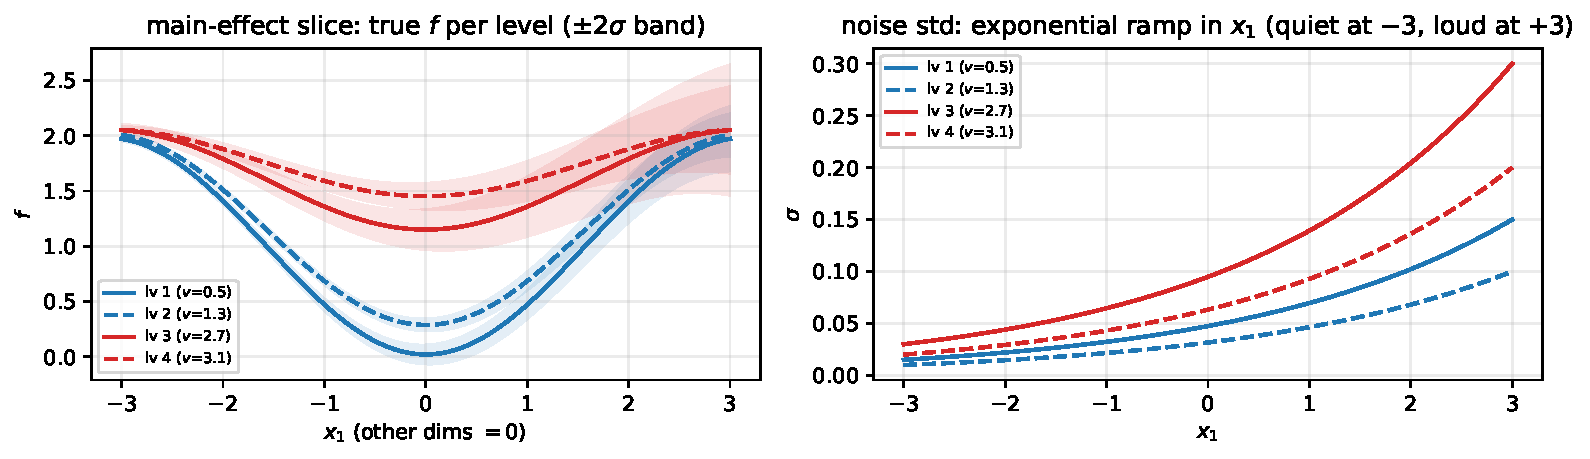
\includegraphics[width=0.9\linewidth]{figs/griewank_truth.pdf}
\caption{Griewank 6-D (v3.1, domain $[-3,3]^5$): main-effect slice along $x_1$; levels form two
pairs $\{0.5,1.3\}$ and $\{2.7,3.1\}$ (solid/dashed = pair members) separated by per-level
offsets $b(\ell)\in\{0,0.15,0.6,0.75\}$, with cluster-split noise multipliers $\{1.5,1.0\}$ vs
$\{3.0,2.0\}$ and the exponential-ramp noise $0.01\cdot10^{(x_1+3)/6}m(\ell)$ (quiet at
$x_1=-3$, up to $\sigma=0.30$ at $+3$).}
\end{figure}
\begin{figure}[htbp]
\centering
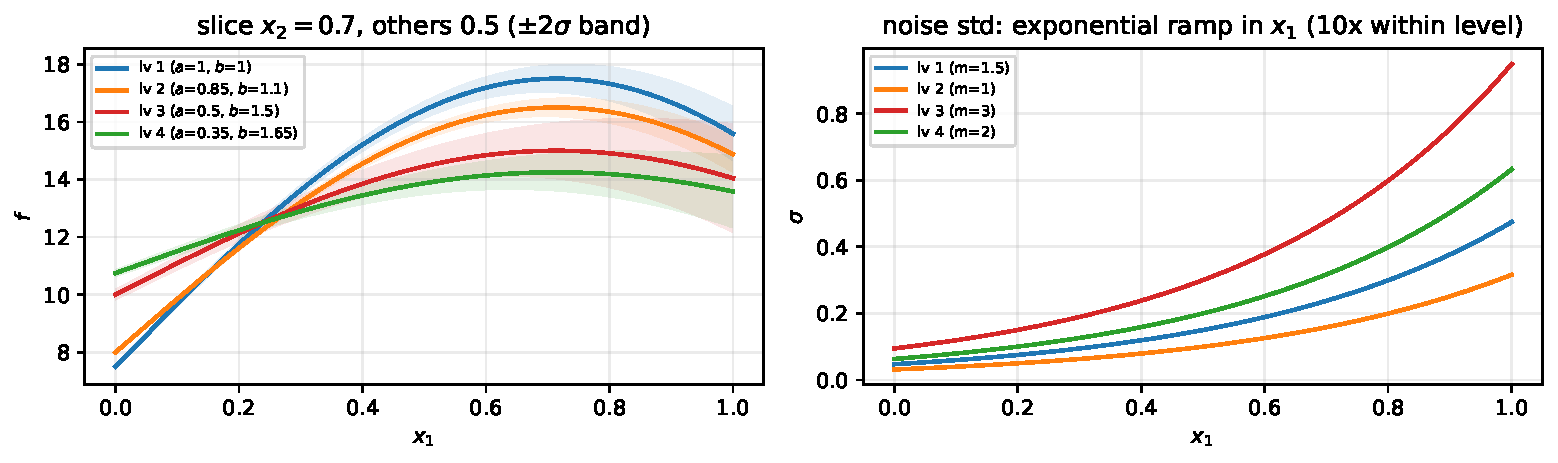
\includegraphics[width=0.9\linewidth]{figs/friedman_truth.pdf}
\caption{Friedman 5-D + categorical (TP-8, \emph{candidate --- single-seed pilot only}):
levels scale the interaction amplitude $a(\ell)\in\{1.0,0.85,0.5,0.35\}$ and the $x_4$
slope $b(\ell)\in\{1.0,1.1,1.5,1.65\}$ --- shape-only pairs $\{1,2\}$/$\{3,4\}$
(within-pair curve RMS 0.65/0.66, cross-pair 1.65--2.88), no constant offsets. Noise:
exponential ramp $0.1\cdot10^{x_1-0.5}m(\ell)$, $m\in\{1.5,1.0,3.0,2.0\}$.}
\end{figure}
\clearpage
